\documentclass[12pt,margin=0px]{article}

\usepackage{subcaption}
\usepackage{multirow}
\usepackage{listings}
\usepackage{hhline}
\usepackage{graphicx}
\usepackage{float}
\usepackage{fancyhdr}
\usepackage{amsthm}
\usepackage{amssymb}
\usepackage{amsmath}
\usepackage{makecell}
\usepackage[utf8]{inputenc}
\usepackage[thinlines]{easytable}
\usepackage[table,xcdraw]{xcolor}
\usepackage[normalem]{ulem}
\usepackage[a4paper, margin=1in]{geometry}
\usepackage{enumitem}
\usepackage{xcolor}

\newcommand\ddfrac[2]{\frac{\displaystyle #1}{\displaystyle #2}}
\definecolor{mygray}{rgb}{0.15, 0.15, 0.15}

\setlist[itemize,1]{label=$\bullet$}
\setlist[itemize,2]{label=$\circ$}
\setlist[itemize,3]{label=$\centerdot$}
\setlist[itemize,4]{label=$\cdot$}

\pagestyle{fancy}

\newcommand\blfootnote[1]{%
  \begingroup
  \renewcommand\thefootnote{}\footnote{#1}%
  \addtocounter{footnote}{-1}%
  \endgroup
}

\renewcommand{\figurename}{ábra}
\newenvironment{tetel}[1]{\paragraph{#1 \\}}{}

\newcommand{\N}{\mathbb{N}}
\newcommand{\Z}{\mathbb{Z}}
\newcommand{\R}{\mathbb{R}}
\newcommand{\Q}{\mathbb{Q}}
\newcommand{\C}{\mathbb{C}}

\makeatletter
\renewcommand\paragraph{%
	\@startsection{paragraph}{4}{0mm}%
	{-\baselineskip}%
	{.5\baselineskip}%
	{\normalfont\normalsize\bfseries}}
\makeatother

% A dokument itt kezdődik
\newcommand\lword[1]{\leavevmode\nobreak\hskip0pt plus\linewidth\penalty50\hskip0pt plus-\linewidth\nobreak #1}
\useunder{\uline}{\ul}{}
\fancyhead{}
\cfoot{9. tétel | \thepage. oldal}

\renewcommand{\headrulewidth}{0pt}
\renewcommand{\footrulewidth}{0.4pt}

\begin{document}
    \thispagestyle{fancy}
    \hyphenation{oddword}
    \uchyph=0

    \begin{center}
        {\huge\bfseries\noindent 9. Programok fordítása és végrehajtása} \\
    \end{center}
	
\section*{Bevezetés}
	
	Amikor programot írunk, azt valamilyen programozási nyelven tesszük. Ezt a programozási nyelvtől függvényében vagy lefordítjuk a gép által értelmezhető kódra, vagy interpreterrel futtatjuk azt.
	
\section*{Fordítás és Interpretálás}
	
\subsection*{Fordítás}
	
    A fordítás során általában egy magas szintű programozási nyelvből gépi kód keletkezik, amelyet a processzor már képes értelmezni és futtatni.\\

    \noindent A következő elönyei vannak:
    \begin{itemize}
        \item \textbf{Gyors}, mivel a lexikális, szintaktikus és szemantikus elemzés fordítási időben, egyszer fut le, valamint ekkor optimalizáljuk a kódot.
        \item \textbf{Fordítási időben sok hibát ki lehet szűrni}, ezáltal megkönnyítve a hibakeresést (debuggolást).
        \item A gépi kód \textbf{nehezen visszafejthető}. (Reverse-engineering nehézkes)
    \end{itemize}
    Általában nagyobb programokhoz használjuk, ahol fontos a hatékonyság. A lefordított kódon később már nem (vagy csak nagyon nehezen) tudunk változtatni.\\
	
	\noindent Hátránya, hogy a keletkezett kód nem platformfüggetlen, minden architektúrára külön-külön le kell fordítani.\\
	
	\noindent \textbf{Például}: C, C++, Ada, Haskell
	
	\begin{figure}[H]
		\centering
		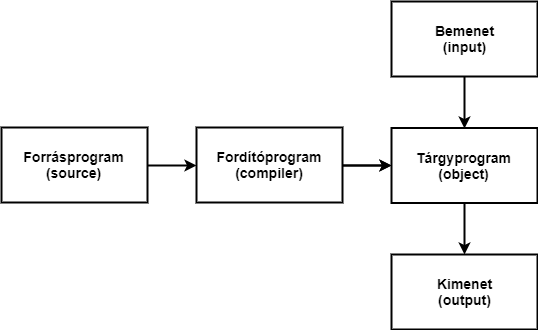
\includegraphics[width=0.55\textwidth]{img/forditas_folyamatabra.png}
		\caption{A fordítás folyamata}
		\label{fig:forditas_folyamatabra}
	\end{figure}
	
	
\subsection*{Interpretálás}
	
	Az interpretálás során az értelmező a programkódot futás közben hajtja végre.\\

    \noindent A következő elönyei vannak:
    \begin{itemize}
        \item Az interpretert mindössze \textbf{egyszer kell csak megírni} az adott rendszerre.
        \item \textbf{Platformfüggetlen}.
    \end{itemize}

    \noindent Hátránya, hogy \textbf{nehéz} benne \textbf{a hibakeresés}. Sok olyan hiba maradhat a kódban, amit egy fordító kiszűrt volna (pl. típus egyezőség).\\
	
	\noindent \textbf{Például}: PHP, JavaScript, ShellScript

	\begin{figure}[H]
		\centering
		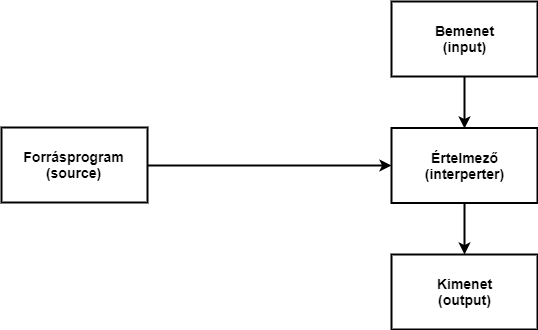
\includegraphics[width=0.5\textwidth]{img/interpretalas_folyamatabra.png}
		\caption{Az interpretálás folyamata}
		\label{fig:interpretalas_folyamatabra}
	\end{figure}
	
	
\subsection*{Fordítás és Interpretálás együtt}
		
    Egyes nyelvek (pl. Java) előfordítást használnak, melynek eredménye a \textit{bájtkód}, amely gépi kód egy virtuális gép számára.\\

    \noindent A következő elönyei vannak:
    \begin{itemize}
        \item Elérhető a \textbf{fordítási idejű hibaellenőrzés és optimalizálás}.
        \item \textbf{Platformfüggetlenség}.
    \end{itemize}
	
	\begin{figure}[H]
		\centering
		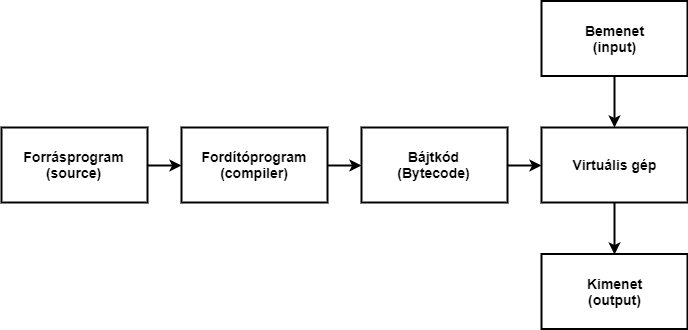
\includegraphics[width=0.6\textwidth]{img/bajtkod_folyamatabra.png}
		\caption{Az interpretálás folyamata}
		\label{fig:bajtkod_folyamatabra}
	\end{figure}
	
    \section*{Fordítási egység és a szerkesztés}

    \noindent Fordítási egység a nyelvnek az az egysége, amely a fordítóprogram egyszeri lefuttatásával, a program többi részétől elkülönülten lefordítható. Ha programunkat fordítási egységekre tagoljuk, akkor elkerülhetjük azt, hogy egyetlen kisebb módosítás miatt a teljes programot újra kelljen fordítani.\\

    \noindent Mivel a fordító a neki átadott forrásfájlokat teljes egészében feldolgozza, ezért a fordítási egységeket úgy tudjuk kialakítani, hogy a forrásprogramot nem egy fájlban helyezzük el, hanem fordítási egységenként tagoljuk. Ezzel a módszerrel egyből a forráskód logikai tagolása is megtörténik, így a forrásszöveg könnyebben áttekinthetővé és megérthetővé válik.\\
	
    \noindent A tárgykód létrehozása két fázisban történik.
    \begin{itemize}
        \item Először a forrásfájlokat \textit{lefordítjuk}, ebből keletkezik az un. \textit{objektumkód} (pl.: .obj, .class). Ebben a gépi utasítások már megvannak, de hiányznak belőle a hivatkozások (pl változók, függvények), melyek más fájlokban vannak megvalósítva.
        \textit{Fordítási egységnek} nevezzük azt, amiből egy objektumkód keletkezik.
	
        \item Második lépésben a \textit{linker} (szerkesztő) feladata, hogy a hiányzó referenciákat kitöltse, hogy egyetlen fájlt generálva futtatható kódot kapjunk.\\\\
        \noindent A linkelés lehet:
        \begin{itemize}
            \item \textbf{Statikus}: az object fájlokat fordítási időbe összeszerkesztjük a könyvtárakkal.
            \item \textbf{Dinamikus}, betöltéskor (load-time): fordítási időben úgynevezett import könyvtárakat használunk, ezek a megosztott könyvtárakra vonatkozó hivatkozásokat tartalmaznak, amiket majd az operációs rendszer a program betöltésekor kapcsol hozzá a futtatható fájlhoz. Ha valamelyik hivatkozott megosztott könyvtár hiányzik, a programot nem lehet betölteni.
            \item \textbf{Dinamikus, futtatáskor} (run-time): fordítási időben a megosztott könyvtárak betöltésére és az eljárások címeinek lekérdezésére vonatkozó rendszerhívások kerülnek a programba. A megosztott könyvtárak betöltése futás közben történik, amikor szükség van rájuk. Ezzel a megoldással lehetőség van arra, hogy a program a neki megfelelő verziójú könyvtárat megkeresse, vagy például a program indításkor ellenőrizze, hogy van-e egyáltalán ilyen.        \end{itemize}
    \end{itemize}	

    \section*{A fordítóprogram komponensei}	

	\begin{figure}[H]
		\centering
		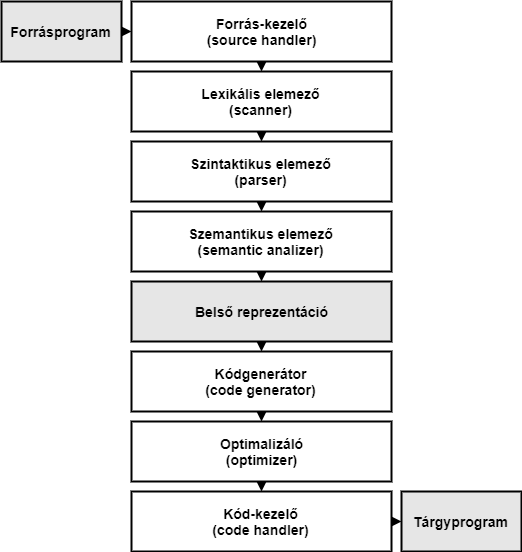
\includegraphics[width=0.6\textwidth]{img/forditas_teljes_folyamata.png}
		\caption{A fordítás lépései}
		\label{fig:forditas_teljes_folyamatabra}
	\end{figure}

    \subsection*{Lexikális elemző}

    \noindent A lexikális elemző feladata, hogy tokenekre bontsa a forráskódot.
	
    \begin{itemize}
        \item Bemenete maga a forráskód.
        \item Adott egy a nyelvre jellemző reguláris (hármas típusú) nyelvtan. Ez adja meg, hogy milyen típusú tokenek szerepelhetnek a forrásban.
        A tokenekhez tulajdonságokat rendelhet (pl. változó neve, literál értéke).
        \item Kimenete ez a tokensorozat. Amennyiben az elemző olyan karaktersorozatot talál, amelynek nem feleltethető meg token, akkor az lexikális hibát vált ki.
    	
        \textit{Megjegyzés: Lexikális hibánál nem feltétlen szakad meg a fordítás folyamata, megpróbálhatjuk átugrani az adott részt és folytatni az elemzést, így ha több hiba is van, akkor azokat egyszerre jelezhetjük.}
    \end{itemize}

    \noindent A reguláris kifejezéseket \emph{véges determinisztikus automatákkal} ismerjük fel.\\

    \noindent Amennyiben egy lexikális elemre az egyik automata elfogadó állapotba kerül, úgy felismertünk egy tokent. Egy karaktersorozatot egyszerre több automata is felismerhet.\\

    \noindent Ha a felismert tokenek \emph{azonos hosszúak}, akkor \emph{a nyelv konfliktusos}. Ennek nem szabad előfordulnia. Az viszont lehetséges, hogy egy szót, és az ő prefixét is felismerte egy automata. Ekkor mindig a hosszabbat választjuk.
	
\subsection*{Szintaktikus elemző}

    A szintaxis elemző bemenete a lexikális elemző kimenete. \\\\
    Feladata, hogy
    \begin{itemize}
        \item \textit{szintaxisfát} építsen a tokenekből, a nyelvez tartozó egy környezetfüggetlen (kettes típusú) grammatika alapján, vagy ha ez lehetetlen, akkor
        \item jelezze ezt \emph{szintaktikus hibaként}.
    \end{itemize}
	
\subsubsection*{LR0 elemzés}
	
	A lexikális elemző által előállított szimbólumsorozatot balról
	jobbra olvassuk, a szimbólumokat az elemző vermébe tesszük.
    \begin{itemize}	
	   \item \emph{Léptetés}: egy új szimbólumot teszünk a bemenetről a verem tetejére.
	   \item \emph{Redukálás}: a verem tetején lévő szabály-jobboldalt helyettesítjük a szabály bal oldalán álló nemterminálissal
	\end{itemize}
	\noindent A háttérben egy véges determinisztikus automata működik:
	az automata átmeneteit a verem tetejére kerülő szimbólumok határozzák meg
	ha az automata végállapotba jut, redukálni kell
	egyéb állapotban pedig léptetni.
	
	\noindent Az automata bizonyos nyelvek esetén konfliktusos lehet: nem tudjuk eldönteni, hogy léptessünk vagy redukáljunk.
	
    \subsubsection*{LR1 elemzés}
	
	\noindent Az előző problémára kínál megoldást, kibővítve a lehetséges nyelvek halmazát.
	
	\noindent Az ötlet, hogy \emph{olvassunk előre} egy szimbólumot.
	
	\noindent Ha az aktuális állapot \emph{i}, és az előreolvasás eredménye az \emph{a} szimbólum:
	\begin{itemize}
	\item ha $ [A	\rightarrow \alpha.a\beta, b] \in I_i $ és $read(I_i, a) = I_j$
	akkor léptetni kell, és átlépni a \emph{j} állapotba.
	
	\item ha $ [A	\rightarrow \alpha., a] \in I_i (A \neq S'), $
	akkor redukálni kell az $ A \rightarrow \alpha $ szabály szerint.
	
	\item ha $ [S' \rightarrow S., \#] \in I_i $ és $ a = \# $, akkor el kell fogadni a szöveget,	minden más esetben hibát kell jelezni.
	
	Ha az \emph{i} állapotban \emph{A} kerül a verem tetejére:		
    ha\ $read(I_i,A) =	I_j$, akkor át kell lépni a \emph{j} állapotba,	egyébként hibát kell jelezni.
    \end{itemize}
	
\subsubsection*{Jelmagyarázat/Kanonikus halmazok}
	
	\paragraph{Closure/lezárás}
	
	\noindent Ha $ I $ a grammatika egy $ LR(1) $ elemhalmaza, akkor $ closure(I) $ a	legszűkebb olyan halmaz, amely az alábbi tulajdonságokkal rendelkezik:
	
	$I \subseteq closure(I) $ ha $ [A \rightarrow \alpha.B\gamma,a] \in closure(I)$,
	és $ B \rightarrow \beta $ a grammatika egy szabálya, akkor $ \forall b \in FIRST1(\gamma{}a) $ esetén $ [B \rightarrow .\beta,b] \in closure(I) $
	
	\paragraph{Read/olvasás}
	Ha $ I $ a grammatika egy $ LR(1) $ elemhalmaza, $ X $ pedig terminális	vagy nemterminális szimbóluma, akkor $ read(I, X) $ a legszűkebb olyan halmaz, amely az alábbi tulajdonsággal rendelkezik:
	Ha $ [A \rightarrow \alpha. X\beta,a] \in I $, akkor $ closure([ A \rightarrow \alpha X.\beta,a]) \subseteq read(I, X) $.
	
	\paragraph{LR(1) kanonikus halmazok ($ I_n $)}
	\begin{itemize}
		\item
		$ closure([S' \rightarrow .S, \#]) $ a grammatika egy kanonikus halmaza.
		\item
		Ha $ I $ a grammatika egy kanonikus elemhalmaza, $ X $ egy terminális vagy nemterminális szimbóluma, és $ read(I, X) $ nem üres, akkor $ read(I, X) $ is a grammatika egy kanonikus halmaza.
		\item
		Az első két szabállyal az összes kanonikus halmaz előáll.
	\end{itemize}
	
\subsection*{Szemantikus elemző}
	

	A szemantikus elemzés jellemzően a környezetfüggő ellenőrzéseket
	valósítja meg.
	
	%Dévai diáiról
	\begin{itemize}
		\item
		deklarációk kezelése: változók, függvények, eljárások, operátorok, 	típusok
		\item
		láthatósági szabályok
		\item
			aritmetikai ellenőrzések
		\item
		a program szintaxisának környezetfüggő részei
		\item
		típusellenőrzés
		\item
		stb.
	\end{itemize}
	
	
    \noindent A szemantikus elemzéshez ki kell egészítenünk a grammatikát. Rendeljünk a szimbólumokhoz attribútumokat és a szabályokhoz akciókat! Egy adott szabályhoz tartozó feltételek csak a szabályban	előforduló attribútumoktól függhetnek.	(Ha egy feltétel nem teljesül, akkor szemantikus hibát kell	jelezni!). A szemantikus rutinok csak annak a szabálynak az	attribútumait használhatják és számíthatják ki, amelyikhez az őket reprezentáló akciószimbólum tartozik. Minden szintaxisfában minden attribútumértéket pontosan egy
	szemantikus rutin határozhat meg. Az így létrejövő nyelvtant \emph{\textbf{attribútum fordítási grammatikának}} (ATG) hívjuk.

	\noindent A \emph{jól definiált attribútum fordítási grammatika}, olyan attribútum fordítási grammatika, amelyre igaz, hogy a	grammatika által definiált nyelv mondataihoz tartozó minden szintaxisfában minden attribútum értéke egyértelműen kiszámítható.
\newpage	
	\noindent Egy attribútumot kétféleképpen lehet meghatározni:
    \begin{itemize}	
	   \item\noindent \textbf{Szintézissel}: a szintaxisfában alulról felfelé terjed az információ, egy szülő attribútumát a gyerekekből számoljuk. Kitüntetettnek hívjuk azokat az attribútumokat, melyeket a lexikális elemző szolgáltat.
	   \item \textbf{Öröklődéssel}: a szintaxisfában felülről lefelé terjed az információ. A gyerekek attribútumait a szülőé határozza meg.
	\end{itemize}
	\noindent Az \emph{L-ATG} olyan attribútum fordítási grammatika, amelyben minden
	$ A	\rightarrow	X_1X_2 . . .	X_n  $szabályban az attribútumértékek az alábbi sorrendben meghatározhatók:
	
	\begin{itemize}
		\item
		A örökölt attribútumai
		\item
		$ X_1 $ örökölt attribútumai
		\item
		$ X_1 $ szintetizált attribútumai
		\item
		$ X_2 $ örökölt attribútumai
		\item
		$ X_2 $ szintetizált attribútumai
		\item
		\dots
		\item
		$ X_n $ örökölt attribútumai
		\item
		$ X_n $ szintetizált attribútumai
		\item
		A szintetizált attribútumai
	\end{itemize}

	\noindent Amennyiben a nyelvtanunk ennek eleget tesz, úgy hatékonyan meghatározható minden attribútum.

    \noindent A szemantikus elemzéshez jellemzően szimbólumtáblát használunk, verem szerkezettel és keresőfával vagy hash-táblával. Minden blokk egy új szint a veremben, egy szimbólum keresése a verem tetejéről indul.
	
    % Kódgenerálás assemblyben alapvető imperatív vezérlési szerkezetekhez.
    \section*{Kódgenerálás alapvető vezérlési szerkezetekhez}


	A kódgenerálás feladata, hogy a szintaktikusan és szemantikusan elemzett programot tárgykóddá alakítsa. Általában szorosan összekapcsolódik a
	szemantikus elemzéssel.
\newpage	
    \subsection*{Értékadás}
	
	\noindent assignment $ \rightarrow $ \emph{variable} \textbf{assignmentOperator} \emph{expression}\\

    \noindent // a kifejezést az eax regiszterbe kiértékelő kód\\
	\noindent \texttt{mov [variable],eax}
	
    \subsection*{Egy ágú elágazás}
	
    \noindent statement $ \rightarrow $ \textbf{if} condition \textbf{then} program \textbf{end}\\
	
    \noindent // a feltételt az al regiszterbe kiértékelő kód\\
    \texttt{
	cmp al,1\\
	je Then\\
	jmp End\\
	Then: \\
    }
    // a then-ág programjának kódja\\
    \texttt{
	End:\\
    }
	
	\noindent \emph{Megjegyzés}: a dupla ugrásra azért van szükség, mert a feltételes ugrás hatóköre limitált.

    \subsection*{Több ágú elágazás}
	
	statement $ \rightarrow $
	\\if $ condition_1 $ then $ program_1 $
	\\elseif $ condition_2 $ then $ program_2 $
	\\\dots
	\\elseif $ condition_n $ then $ program_n $
	\\else $ program_{n+1} $ end\\
	
    \noindent // az 1. feltétel kiértékelése az al regiszterbe\\
    \texttt{
    cmp al,1\\
    jne near Condition\_2\\
    }
    // az 1. ág programjának kódja\\
    \texttt{
    jmp End\\
    ...\\
    }
    //az n-edik feltétel kiértékelése az al regiszterbe\\
    \texttt{
    Condition\_n: \\
    cmp al,1\\
    jne near Else\\
    }
    // az n-edik ág programjának kódja\\
    \texttt{
    jmp End\\
    Else:\\
    }
    // az else ág programjának kódja\\
    \texttt{
    End:
    }

    \subsection*{Switch-case}

	statement $ \rightarrow $ \textbf{switch} \emph{variable}
	\\case $ value_1 $ : $ program_1 $
	\\...
	\\case $ value_n $ : $ program_n $\\

    \noindent \texttt{cmp [variable], value\_1\\
    je near Program\_1\\
    cmp [variable], value\_2\\
    je near Program\_2\\
    . ..\\
    cmp [variable], value\_n\\
    je near Program\_n\\
    jmp End\\
    Program\_1:\\
    }
    // az 1. ág programjának kódja\\
    \texttt{
    . ..\\
    Program\_n:\\
    }
    // az n-edik ág programjának kódja\\
    \texttt{
    End:
    }

    \subsection*{Ciklus}

    \subsubsection*{Elől tesztelő}	

	statement $ \rightarrow $ \textbf{while} \emph{condition} statements \textbf{end}\\
	
	\noindent \texttt{Begin:}\\
    //a ciklusfeltétel kiértékelése az al regiszterbe\\
	\texttt{cmp al,1\\
	jne near End}\\
	// a ciklusmag programjának kódja\\
	\texttt{jmp Begin\\
	End:}
	
    \subsubsection*{Hátul tesztelő}	
	statement $ \rightarrow $ loop statements \textbf{while} \emph{condition}\\

	\noindent
    \texttt{Begin: }\\
    //a ciklusmag programjának kódja\\
    . ..\\
	//a ciklusfeltétel kiértékelése az al regiszterbe\\
    \texttt{
    cmp al,1\\
	je near Begin
    }
	
\subsubsection*{For ciklus}	

	statement $ \rightarrow $ \textbf{for} variable \textbf{from} $ value_1 $ to $ value_2 $ statements \textbf{end}\\
	
	\noindent // a "from" érték kiszámítása a [Változó] memóriahelyre\\
	\texttt{Begin: }\\
    // a "to" érték kiszámítása az eax regiszterbe\\
	\texttt{cmp [variable],eax\\
	ja near End}\\
	// a ciklusmag kódja\\
	\texttt{inc [variable]\\
	jmp Begin\\
	End:}

\subsection*{Statikus változók}
	
	Kezdőérték nélküli változódefiníció fordítása:\\

	\noindent \texttt{section .bss}\\
    // a korábban definiált változók...\\
    \texttt{Lab12: resd 1 ; 1 x 4 bájtnyi terület}\\
	
	\noindent Kezdőértékkel adott változódefiníció fordítása:\\

	\noindent \texttt{section .data}\\
	// a korábban definiált változók...\\
	\texttt{Lab12: dd 5 ; 4 bájton tárolva az 5-ös érték}

    \subsection*{Logikai kifejezések}

    \subsubsection*{kifejezés1 $ < $  kifejezés2 }
	
	// a 2. kifejezés kiértékelése az eax regiszterbe\\
	\texttt{push eax}\\
	// az 1. kifejezés kiértékelése az eax regiszterbe\\
	\texttt{pop ebx\\
	cmp eax,ebx\\
	jb Smaller\\
	mov al,0 } // hamis\\
	\texttt{jmp End\\
	Smaller:\\
	mov al,1 }// igaz\\
	\texttt{End:}
\newpage
    \subsubsection*{kifejezés1 $ \lbrace $ és, vagy, nem, kizáróvagy  $ \rbrace $  kifejezés2 }

	// a 2. kifejezés kiértékelése az al regiszterbe\\
	\texttt{push ax} ; nem lehet 1 bájtot a verembe tenni!\\
	// az 1. kifejezés kiértékelése az al regiszterbe\\
	\texttt{pop bx} ; // bx-nek a bl részében van,\\
	// ami nekünk fontos\\
	\texttt{and al, bl}\\
	
    \subsubsection*{ lusta "és" kiértékelés }
	
	// az 1. kifejezés kiértékelése az al regiszterbe\\
	\texttt{cmp al,0\\
	je End\\
	push ax}\\
	// a 2. kifejezés kiértékelése az al regiszterbe\\
	\texttt{mov bl,al\\
	pop ax\\
	and al,bl\\
	End:}

    \subsubsection*{ Alprogramok megvalósítása }
	
	
	// az 1. kifejezés kiértékelése az al regiszterbe\\
    \texttt{
    cmp al,0\\
	je End\\
	push ax}\\
	// a 2. kifejezés kiértékelése az al regiszterbe\\
    \texttt{
    mov bl,al\\
	pop ax\\
	and al,bl\\
	End:}
	
    \subsubsection*{ Alprogramok hívása }

	// Alprogramok sémája\\
	// utolsó paraméter kiértékelése eax-be\\
	\texttt{push eax}\\
	// ...\\
	// 1. paraméter kiértékelése eax-be\\
	\texttt{push eax\\
	call alprogram\\
	add esp,’a paraméterek összhossza’}
\newpage	
    \section*{Kódoptimalizáló}
	
    Az optimalizálás feladata, hogy a keletkezett kód kisebb és gyorsabb legyen, úgy hogy a futás eredménye nem változik. A gyorsaság és a tömörség gyakran ellentmondanak egymásnak, és az egyik csak a másik rovására javítható.\\
    
    \noindent Általában három lépésben szokás elvégezni:
	
	\begin{itemize}
		\item
		Optimalizálási lépések végrehajtása az eredeti programon, vagy egyszerűsített változatán
		\item
		Kódgenerálás
		\item
		Gépfüggő optimalizálás végrehajtása a generált kódon
	\end{itemize}
	
    \subsection*{Lokális optimalizáció}
	
    \noindent Egy programban egymást követő utasítások sorozatát \emph{alapblokknak} nevezzük,
    \begin{itemize}
        \item ha az első utasítás kivételével egyik utasítására sem lehet távolról átadni a vezérlést
        \begin{itemize}
            \item assembly programokban: ahová a \textbf{jmp}, \textbf{call}, \textbf{ret} utasítások "ugranak" 
            \item magas szintű nyelvekben: \emph{eljárások és ciklusok eleje}, \emph{elágazások ágainak első utasítása}, \emph{goto utasítások célpontjai}.
        \end{itemize}
        \item az utolsó utasítás kivételével nincs benne vezérlés-átadó utasítás 
        \begin{itemize}
            \item assembly programokban: ahová a \textbf{jmp}, \textbf{call}, \textbf{ret} utasítások "ugranak" 
            \item magas szintű nyelvekben: \emph{elágazások és ciklusok vége}, \emph{eljárás vége}, \emph{goto utasítások célpontjai}.
        \end{itemize}
    \end{itemize}
    
    \noindent Az utasítás-sorozat nem bővíthető a fenti két szabály megsértése nélkül.\\
	
    \noindent Jelöljük meg:
    \begin{itemize}
        \item a program első utasítását
        \item azokat az utasításokat, amelyekre távolról át lehet adni avezérlést
        \item a vezérlés-átadó utasításokat követő utasításokat
    \end{itemize}

    \noindent Minden megjelölt utasításhoz tartozik egy alapblokk, ami a következő megjelölt utasításig (vagy az utolsó utasításig) tart.\\

    \noindent \textbf{main: mov eax,[Label1]}\\
        \texttt{cmp eax,[Label2]}\\
        \texttt{jz True}\\
        \textbf{dec dword [Label1]}\\
        \texttt{inc dword [Label2]}\\
        \texttt{jmp vege}\\
    \textbf{True: inc dword [Label1]}\\
        \texttt{dec dword [Label2]}\\
    \textbf{End: ret}

	\noindent Ha az optimalizálás az alapblokkok keretein belül történik, akkor garantált, hogy az átalakításnak nincs mellékhatása. Ez a \emph{lokális optimalizálás}.\\

    \paragraph*{Tömörítés}

    \noindent Cél: minél kevesebb konstans és konstans értékű változó legyen.\\
    \noindent Konstansok összevonása: a fordítási időben kiértékelhető kifejezések kiszámítása.\\

    \noindent \emph{Eredeti kód}: \texttt{a := 1 + b + 3 + 4;}\\
    \noindent \emph{Optimalizált kód}: \texttt{a := 8 + b;}\\
	
    \noindent \emph{Eredeti kód}:\\
    \texttt{a := 6;}\\
    \texttt{b := a / 2;}\\
    \texttt{c := b + 5;}\\

    \noindent \emph{Optimalizált kód}:\\
    \texttt{a := 6;}\\
    \texttt{b := 3;}\\
    \texttt{c := 8;}\\

    \noindent \emph{Eredeti kód}:\\
    \texttt{x := 20 - (a * b);}\\
    \texttt{y := (a * b) \^\ 2;}\\

    \noindent \emph{Optimalizált kód}:\\
    \texttt{t := a * b;}\\
    \texttt{x := 20 - t;}\\
    \texttt{y := t \^\ 2;}\\

	\paragraph{Ablakoptimalizálás}

    \noindent Ez egy módszer a lokális optimalizálás egyes fajtáihoz. Egyszerre csak néhány utasításnyi részt vizsgálunk a kódból. A vizsgált részt előre megadott mintákkal hasonlítjuk össze. Ha illeszkedik, akkor a mintához megadott szabály szerint átalakítjuk ezt az "ablakot" végigcsúsztatjuk a programon. Az átalakítások megadása:

	\begin{center}
	$ \lbrace$ minta $ \rightarrow $ helyettesítés $\rbrace$ szabályhalmazzal\\
	(a mintában lehet paramétereket is használni)
	\end{center}

	\noindent Példák:
	\begin{itemize}
		\item
		felesleges műveletek törlése: nulla hozzáadása vagy kivonása
		\item
		egyszerűsítések: nullával szorzás helyett a regiszter törlése
		\item
		regiszterbe töltés és ugyanoda visszaírás esetén a visszaírás elhagyható
		\item
		utasításismétlések törlése: ha lehetséges, az ismétlések törlése
	\end{itemize}
\newpage    
    \noindent Példa: \\
    
    \noindent Ablak mérete: 1 utasítás\\
    Szabályhalmaz:\\
    \{\texttt{mov reg,0 $\to$ xor reg,reg},\\
    \texttt{add reg,0 $\to$ elhagyható}\}\\
	
    \noindent \emph{Eredeti kód}:\\
    \texttt{add eax,0}\\
    \texttt{mov ebx,eax}\\
    \texttt{mov ecx,0}\\

    \noindent \emph{Optimalizált kód}:\\
    \texttt{; elhagyott utasítás}\\
    \texttt{mov ebx,eax}\\
    \texttt{xor ecx,ecx}

    \subsection*{Globális optimalizáció}

	A teljes program szerkezetét meg kell vizsgálni. Ennek módszere az adatáram-analízis:
	\begin{itemize}
		\item
		Mely változók értékeit számolja ki egy adott alapblokk?
		\item
		Mely változók értékeit melyik alapblokk használja fel?
	\end{itemize}
	
    \noindent Ez lehetővé teszi az
    \begin{itemize}
        \item azonos kifejezések többszöri kiszámításának kiküszöbölését akkor is, ha különböző alapblokkokban szerepelnek
        \item a konstansok és változók továbbterjesztését alapblokkok között
        \item elágazások, ciklusok optimalizálását
    \end{itemize}

    \paragraph*{Kódkiemelés}
    
\newenvironment{lbmatrix}{\begin{bmatrix*}[l]}{\end{bmatrix*}}    
    
    \noindent \emph{Eredeti kód}:
    \begin{verbatim}
if( x < 10 )
{
    b++;
    a = 0;
}
else
{
    b--;
    a = 0;
}
    \end{verbatim}
\newpage
    \noindent \emph{Optimalizált kód}:\\
    \noindent \textbf{a = 0;}
    \begin{verbatim}
if( x < 10 )
{
    b++;
}
else
{
    b--;
}
    \end{verbatim}

    \section*{A szekvenciális és	párhuzamos/elosztott végrehajtás összehasonlítása}
	
    \subsection*{Szekvenciális végrehajtás:}

    \noindent Ilyenkor a végrehajtás egy processzoron történik. Minden művelet atomi. Egy inputhoz egy output tartozik. Két szekvenciális program ekvivalens, ha ezek a párosok megegyeznek. Nem használja fel az összes rendelkezésre álló erőforrást.

    \subsection*{Párhuzamos végrehajtás:}		

    \noindent Több processzoron hajtódik végre a program. A párhuzamos folyamatok egymással kommunikálva, szinkronban oldják meg az adott problémát. A konkurens program szétbontható elemi szekvenciális programokra, ezek a folyamatok. A folyamatok használhatnak közös erőforrásokat: pl. változók, adattípus  objektumok, kommunikációs csatornák.
	
	\noindent A kommunikációt általában kétféleképpen szokták megvalósítani.

	\paragraph{Osztott memóriával.} Ekkor szinkronizálni kell, hogy ki mikor fér hozzá, hogy ne legyen ütközés.

    \paragraph{Kommunikációs csatornával.} Garantálni kell, hogy ha egy folyamat üzenetet küld egy másiknak, akkor az meg is kapja azt, és jelezzen is vissza. Ügyelni kell, nehogy deadlock alakuljon ki.
		
\end{document}



